\section{Experiments and results}
\label{sec:experiments_and_results}

\subsection{Data}
\label{sec:data}
\cref{tab:data} summarizes the datasets used for evaluation.

\subsubsection{Public data for simulation}

\ac{T1w} \acp{MRI} were collected from publicly available datasets \ac{IXI}\fnurl{https://brain-development.org/ixi-dataset/}, \ac{ADNI} \cite{jack_alzheimers_2008}, and \ac{OASIS} \cite{lamontagne_oasis-3_2019}, for a total of 1813 images.

These datasets are used as control subjects in our self-supervised experiments (\cref{sec:sim_res_self}).
Although we use the term `control' to refer to subjects that have not undergone resective surgery, they may have other neurological conditions.
For example, subjects in \ac{ADNI} may suffer from Alzheimer's disease.


\newcommand{\zoom}[3]{$ #1 \times #2 \times #3 $}
\newcommand{\mr}[2]{\multirow{#1}{*}{#2}}
\newcommand{\mrsp}[4]{\mr{#1}{\zoom{#2}{#3}{#4}}}

\begin{table}
    \small
    \centering
    \caption{
        Datasets used in this study.
        Where multiple resolutions are present, the minimum, mean and maximum for each dimension are shown.
        `\acs{T1wCE}' indicates that gadolinium was administered for contrast enhancement.
    }
    \label{tab:data}
    \begin{tabular}{lclccc}
        \toprule
        \textbf{Dataset} & \textbf{Modality} & \textbf{Resolution (mm)} & \textbf{Subjects} & \textbf{Surgery} & \textbf{Annotated} \\
        \midrule
        \mr{3}{\textbf{IXI}}     &             \mr{3}{\ac{T1w}} & \zoom{0.94}{0.94}{1.20}  &       \mr{3}{566} &          \mr{3}{-} &          \mr{3}{-} \\
                                 &                           & \zoom{0.94}{0.94}{1.20}  &                   &                    &                    \\
                                 &                           & \zoom{0.98}{0.98}{1.20}  &                   &                    &                    \\
        \midrule
        \textbf{ADNI}            &                     \ac{T1w} & \zoom{1.00}{1.00}{1.00}  &               467 &                  - &                  - \\
        \midrule
        \mr{3}{\textbf{OASIS}}   &             \mr{3}{\ac{T1w}} & \zoom{1.00}{1.00}{1.00}  &       \mr{3}{780} &          \mr{3}{-} &          \mr{3}{-} \\
                                 &                           & \zoom{1.05}{1.01}{1.02}  &                   &                    &                    \\
                                 &                           & \zoom{1.20}{1.05}{3.00}  &                   &                    &                    \\
        \midrule
        \mr{3}{\textbf{EPISURG}} &             \mr{3}{\ac{T1w}} & \zoom{0.75}{0.75}{0.75}  &       \mr{3}{430} &   \mr{3}{Epilepsy} &        \mr{3}{133} \\
                                 &                           & \zoom{0.96}{0.96}{1.08}  &                   &                    &                    \\
                                 &                           & \zoom{1.09}{1.09}{1.60}  &                   &                    &                    \\
        \midrule
        \textbf{Milan}           &                     \ac{T1w} & \zoom{0.46}{0.46}{0.90}  &                20 &           Epilepsy &                 20 \\
        \midrule
        \mr{3}{\textbf{Strasbourg}} &    \mr{3}{\ac{T1w} \& \acs{T1wCE}} & \zoom{0.23}{0.23}{0.50}  &        \mr{3}{33} &   \mr{3}{Epilepsy} &         \mr{3}{33} \\
                                 &                           & \zoom{0.61}{0.61}{2.79}  &                   &                    &                    \\
                                 &                           & \zoom{1.00}{1.00}{5.00}  &                   &                    &                    \\
        \midrule
        \mr{3}{\textbf{Paris}}   &             \mr{3}{\ac{T1w}} & \zoom{0.47}{0.47}{0.49}  &        \mr{3}{19} &   \mr{3}{Epilepsy} &         \mr{3}{19} \\
                                 &                           & \zoom{0.82}{0.76}{1.06}  &                   &                    &                    \\
                                 &                           & \zoom{1.20}{0.98}{1.20}  &                   &                    &                    \\
        \midrule
        \mr{3}{\textbf{BITE}}    &         \mr{3}{\acs{T1wCE}} & \zoom{1.00}{0.47}{0.47}  &        \mr{3}{13} &      \mr{3}{Tumor} &          \mr{3}{0} \\
                                 &                           & \zoom{2.31}{0.53}{0.53}  &                   &                    &                    \\
                                 &                           & \zoom{5.50}{0.55}{0.55}  &                   &                    &                    \\
        \bottomrule
    \end{tabular}
\end{table}



% \subsubsection{EPISURG dataset}
% \label{sec:episurg}

% We curated the EPISURG dataset using images from patients with refractory focal epilepsy who underwent resective surgery between 1990 and 2018 at the \ac{NHNN}, London, United Kingdom.
% These were anonymized data that had been previously acquired as a part of clinical care, so individual patient consent was not required.
% All images in EPISURG were defaced using a predefined face mask in the \ac{MNI} space to preserve patient identity.
% In total, there were 430 patients with postoperative \ac{T1w} \ac{MRI}, 268 of which had a corresponding preoperative \ac{MRI}.
% The distribution of resection types is shown in \tableref{tab:episurg}.

% EPISURG is available online and can be freely downloaded \cite{perez-garcia_episurg_2020}.

% \begin{table}
%     \centering
%     \footnotesize
%     \floatconts
%     {tab:episurg}
%     {\caption{%
%         Distribution of resection types in EPISURG.
%     }}
%     {
%         \begin{tabular}{llr}
%             \toprule
%             \textbf{Lobe}      & \textbf{Type}    & \textbf{Subjects} \\
%             \midrule
%             Temporal           & lobectomy        &        317 \\
%             Temporal           & lesionectomy     &         30 \\
%             Temporal-frontal   & lobectomy        &          2 \\
%             Temporal-parietal  & lobectomy        &          1 \\
%             Frontal            & lobectomy        &         47 \\
%             Frontal            & lesionectomy     &         10 \\
%             Parietal           & lesionectomy     &         11 \\
%             Parietal           & lobectomy        &          4 \\
%             Occipital-parietal & lobectomy        &          2 \\
%             Occipital          & lobectomy        &          2 \\
%             -                  & multiple subpial &          2 \\
%             -                  & hemispherectomy  &          2 \\
%             \midrule
%             \textbf{Total}     &                  &        430 \\
%             \bottomrule
%         \end{tabular}
%     }
% \end{table}

% %Three human raters annotated a subset of the postoperative images in EPISURG \cite{perez-garcia_simulation_2020}.
% Annotations used for evaluation in this study were performed semi-automatically using a fast grow-cut algorithm implemented in 3D Slicer 4.10 \cite{zhu_effective_2014,fedorov_3d_2012}.



% \subsubsection{Multicenter epilepsy data}
% \label{sec:multicenter}

% We evaluate the generalizability of our learning strategy to data from several institutions (\textit{Milan}, \textit{Strasbourg}, \textit{Paris}) that use different acquisition protocols and surgical approaches.
% The same human rater (F.P.G.) annotated all images from these institutions
% %using the same protocol that was used for EPISURG.
% following the same protocol as used for EPISURG.


% \subsubsection{Brain tumor datasets}

% The \ac{BITE} dataset \cite{mercier_online_2012} consists of ultrasound and \ac{MRI} of patients with brain tumors.
% We use the 13 postoperative \ac{T1wCE} in \ac{BITE} to perform a qualitative assessment of the potential of our models to generalize to images from a substantially different domain (images are contrast-enhanced) and different pathology, which may require different surgical techniques that could affect resection cavity appearance.



% \subsubsection{Preprocessing}
% \label{sec:preprocessing}

% For all images, the brain was segmented using ROBEX \cite{iglesias_robust_2011}.
% Voxels within the brain were used to register the images to the nonlinear symmetric ICBM152 \ac{MNI} template \cite{fonov_unbiased_2009,fonov_unbiased_2011} using a pyramidal approach to compute the affine transformation \cite{modat_global_2014}.
% %This registration strategy was robust enough to correctly register the 2347 images used in this work.
% All images were resampled into the \ac{MNI} space using sinc interpolation to preserve image quality.
% After resampling, images had a 1-mm isotropic resolution and size \zoom{193}{229}{193}.



% \subsection{Network architecture and implementation details}
% \subsection{Network architecture and implementation details}

We used the PyTorch deep learning framework \cite{paszke_pytorch_2019}, training with \ac{AMP} on two 32-GB TESLA V100 \acp{GPU}.
In the \ac{AMP} setting, some operations such as convolution are computed using half precision (i.e., 16-bit floating point) to reduce the computational burden while maintaining a similar performance.

We implemented a variant of 3D U-Net \cite{cicek_3d_2016} using two downsampling and upsampling blocks, upsampling with trilinear interpolation for the synthesis path, and 1/4 of the filters for each convolutional layer.
We used dilated convolutions \cite{chen_deeplab_2017}, starting with a dilation factor of one, then increased or decreased in steps of one after each downsampling or upsampling block, respectively.
This results in a model with the same receptive field (a cube of length 88 mm) but $\approx 77 \times$ fewer parameters (\num{246156}) than the original 3D U-Net, reducing overfitting and computational burden.

Convolutional layers were initialized using He's method and followed by batch normalization and nonlinear \ac{PReLU} activation functions \cite{ioffe_batch_2015,he_delving_2015}.
We used adaptive moment estimation (AdamW) \cite{kingma_adam_2014,loshchilov_decoupled_2019} to adjust the learning rate during training, with weight decay of~$10^{-2}$ and a learning scheduler that divides the learning rate by ten every 20 epochs.
We optimized our network to minimize the mean soft Dice loss \cite{milletari_v-net_2016} of each mini-batch, for all the experiments.
A mini-batch size of ten images (five per \ac{GPU}) was used for training.
Self-supervised training took about 27 hours.
Fine-tuning on a small annotated dataset took about seven hours.

We used Sacred \cite{greff_sacred_2017} and TensorBoard \cite{abadi_tensorflow_2016} to configure, log and visualize our experiments.


% \subsection{Processing during training}
% \subsection{Processing during training}

\subsubsection{Resection simulation}

We perform the resection simulation on the fly, i.e., during training.
Simulation requires around 0.5 s for an image of size $193 \times 229 \times 193$.%, depending on the addition of white matter lesions and blood products (\cref{sec:white,sec:blood}).
In practice, we perform expensive operations such as convolutions on subvolumes to reduce computational burden.
The simulation is implemented using SimpleITK \cite{lowekamp_design_2013}, VTK \cite{schroeder_visualization_2006} and NumPy \cite{van_der_walt_numpy_2011}.
To generate the noisy sphere, we used \texttt{pyDome}\fnurl{https://github.com/badassdatascience/pyDome} and \texttt{noise}\fnurl{https://github.com/caseman/noise}.

We use TorchIO transforms to load, preprocess and augment our data during training \cite{perez-garcia_torchio_2020}.
Instead of preprocessing the images with denoising or bias removal, we simulate different artifacts in the training instances so that our models are robust to them.

Our preprocessing and augmentation transforms are described below.
For transforms that are not applied to all images, we show the probability $p$ of the transform being applied.

\begin{enumerate}
    \item Random resection simulation (for self-supervised training only)
    \item Histogram standardization \cite{nyul_new_2000}
    \item Simulation of low resolution artifacts ($p = 0.75$). Sampled uniformly from
    \begin{enumerate}
        \item Random simulation of anisotropic spacing \cite{billot_partial_2020} and
        \item Gaussian blurring with random variance
    \end{enumerate}
    \item Random simulation of MRI ghosting artifacts \cite{shaw_heteroscedastic_2020} ($p = 0.2$)
    \item Random simulation of MRI spike artifacts \cite{shaw_heteroscedastic_2020} ($p = 0.2$)
    \item Random simulation of MRI motion artifacts \cite{shaw_mri_2019} ($p = 0.2$)
    \item Random simulation of bias field inhomogeneity \cite{sudre_longitudinal_2017} ($p = 0.5$)
    \item Foreground standardization to zero-mean and unit variance using only voxels with intensity above the mean to compute the statistics
    \item Gaussian noise with random variance ($p = 0.75$)
    \item Diffeomorphic spatial transform, sampled from either
    \begin{enumerate}
        \item Random rotation and anisotropic scaling ($p = 0.9$) or
        \item Random elastic deformation ($p = 0.1$)
    \end{enumerate}
    \item Random flip around the sagittal plane ($p = 0.5$)
    \item Crop to a tight bounding box around the brain of size of $176 \times 216 \times 160$ voxels.
\end{enumerate}

We refer the reader to the GitHub repository for details on the transforms parameters used for our experiments.



% \subsection{Experiments}

% All overlap measurements are expressed as `median (interquartile range)' \ac{DSC}.
% No postprocessing is performed for evaluation, except thresholding at 0.5.
% We analyzed differences in model performance using a one-tailed Mann-Whitney $U$ test (as \acp{DSC} were not normally distributed) with a significance threshold of $\alpha = 0.05$, and a Bonferroni correction for each set of $N$ experiments: $\alpha\st{Bonf} = \frac{\alpha}{N \times (N - 1)}$.


% \subsubsection{Self-supervised learning: training with simulated resections only}
\label{sec:self}

In our first experiment, we assess the relation between the resection simulation complexity and the segmentation performance of the model.
We train our model with simulated resections on the publicly available dataset $D\pre = \{ \X_{{\pre}_i} \}_{i = 1}^{n\pre}$, where $n\pre = 1813$ (\cref{sec:data}).
We use 90\% of the images in $D\pre$ for the training set $D\st{pre,train}$ and 10\% for the validation set.
At each training iteration, $b$ images from $D\st{pre,train}$ are loaded, resected, preprocessed and augmented to obtain a mini-batch of $b$ training instances
$\{ ( \X_{\text{sim}_i}, \Y_{\text{sim}_i}) \}_{i = 1}^{b}$.
Note that the resection simulation is performed on the fly, which ensures that the network never sees the same resection during training.
Models were trained for 60 epochs, using an initial learning rate of $10^{-3}$.
We use the model weights from the epoch with the lowest mean validation loss obtained during training for evaluation.
Models were tested on the 133 annotated images in EPISURG.

To investigate the effect of the simulated cavity shape on model performance, we modify $\phi\simul$ to generate cuboid- (\cref{fig:exp_shape_cuboid}) or ellipsoid-shaped (\cref{fig:exp_shape_ellipsoid}) resections, and compare with the baseline ``noisy'' ellipsoid (\cref{fig:exp_shape_noisy}).
The cuboids and ellipsoid meshes are not perturbed using simplex noise, and cuboids are not rotated.

Best results were obtained by the baseline model (80.5 (18.7)), trained using ellipsoids perturbed with procedural noise.
Models trained with cuboids and rotated ellipsoids performed significantly (57.9 (73.1), $p < 10^{-8}$) and marginally (79.0 (20.0), $p = 0.123$) worse.

\begin{figure}
  \centering
  \captionsetup[subfigure]{aboveskip=3pt, belowskip=5pt}

  \begin{subfigure}{0.32\textwidth}
    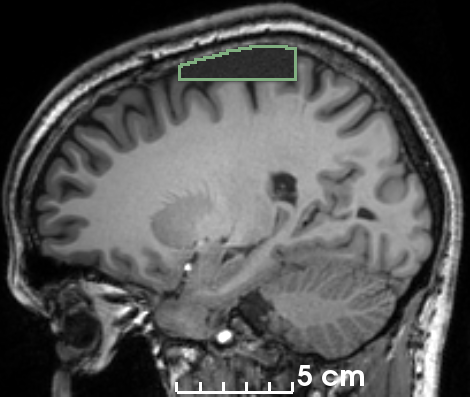
\includegraphics[width=\linewidth]{exp_shape_cuboid}
    \caption{\label{fig:exp_shape_cuboid}}
  \end{subfigure}
  \hfill
  \begin{subfigure}{0.32\textwidth}
    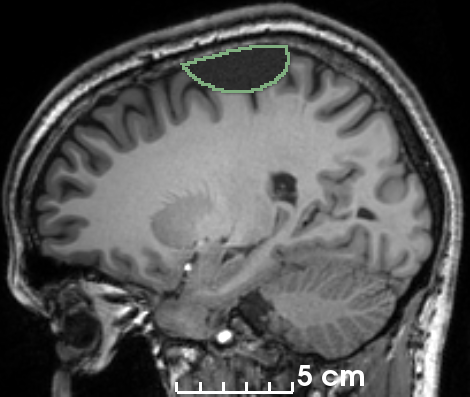
\includegraphics[width=\linewidth]{exp_shape_ellipsoid}
    \caption{\label{fig:exp_shape_ellipsoid}}
  \end{subfigure}
  \hfill
  \begin{subfigure}{0.32\textwidth}
    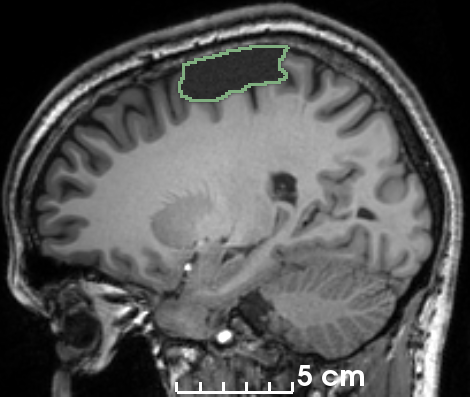
\includegraphics[width=\linewidth]{exp_shape_noisy}
    \caption{\label{fig:exp_shape_noisy}}
  \end{subfigure}

  \caption{
    Simulation of \acp{RC} with increasing shape complexity (\cref{sec:simulation}):
    cuboid (\subref{fig:exp_shape_cuboid}),
    ellipsoid (\subref{fig:exp_shape_ellipsoid})
    and ellipsoid perturbed with simplex noise (\subref{fig:exp_shape_noisy}).
  }
  \label{fig:exp_shape}
\end{figure}

% \subsubsection{Fine-tuning on small clinical datasets}

We assessed the generalizability of our baseline model by fine-tuning it on small datasets from four institutions that may use different surgical approaches and acquisition protocols (including contrast enhancement and anisotropic spacing in \textit{Strasbourg}) (\cref{sec:multicenter}).
Additionally, we fine-tuned the model on 20 cases from EPISURG with the lowest \ac{DSC} in \cref{sec:self}.

For each dataset, we load the pretrained baseline model, initialize the optimizer with an initial learning rate of $5 \times 10^{-4}$, initialize the learning rate scheduler and fine-tune all layers simultaneously for 40 epochs using 5-fold cross-validation.
We use model weights from the epoch with the lowest mean validation loss for evaluation.
To minimize data leakage, we determined the above hyperparameters using the validation set of one fold in the \textit{Milan} dataset.

We observed a consistent increase in \ac{DSC} for all fine-tuned models, up to a maximum of 89.2 (13.3) for the \textit{Milan} dataset.
For comparison, inter-rater agreement between human annotators in our previous study was 84.0 (9.9) \cite{perez-garcia_simulation_2020}.
Quantitative and qualitative evaluations are illustrated in \cref{fig:finetuning_quant,fig:finetuning_qual}, respectively.


\begin{figure}
  \centering
  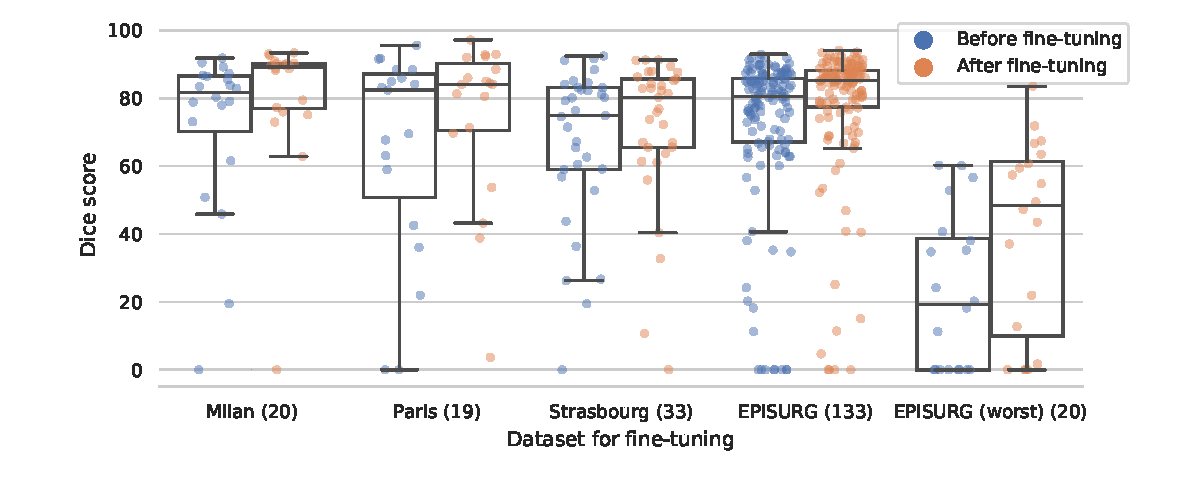
\includegraphics[trim=1cm 0 0.8cm 0, clip, width=\linewidth]{boxplot_finetuning}
  \caption{
    \ac{DSC} without (blue) and with (orange) fine-tuning of the model training using self-supervision.
    Horizontal lines in the boxes represent the first, second (median) and third quartiles.
    The `EPISURG (worst)' dataset comprises the 20 cases from EPISURG with the lowest \ac{DSC} in the experiment described in \cref{sec:self}.
    Numbers in parentheses indicate subjects per dataset.
  }
  \label{fig:finetuning_quant}
\end{figure}


\begin{figure}[ht!]
  \centering
  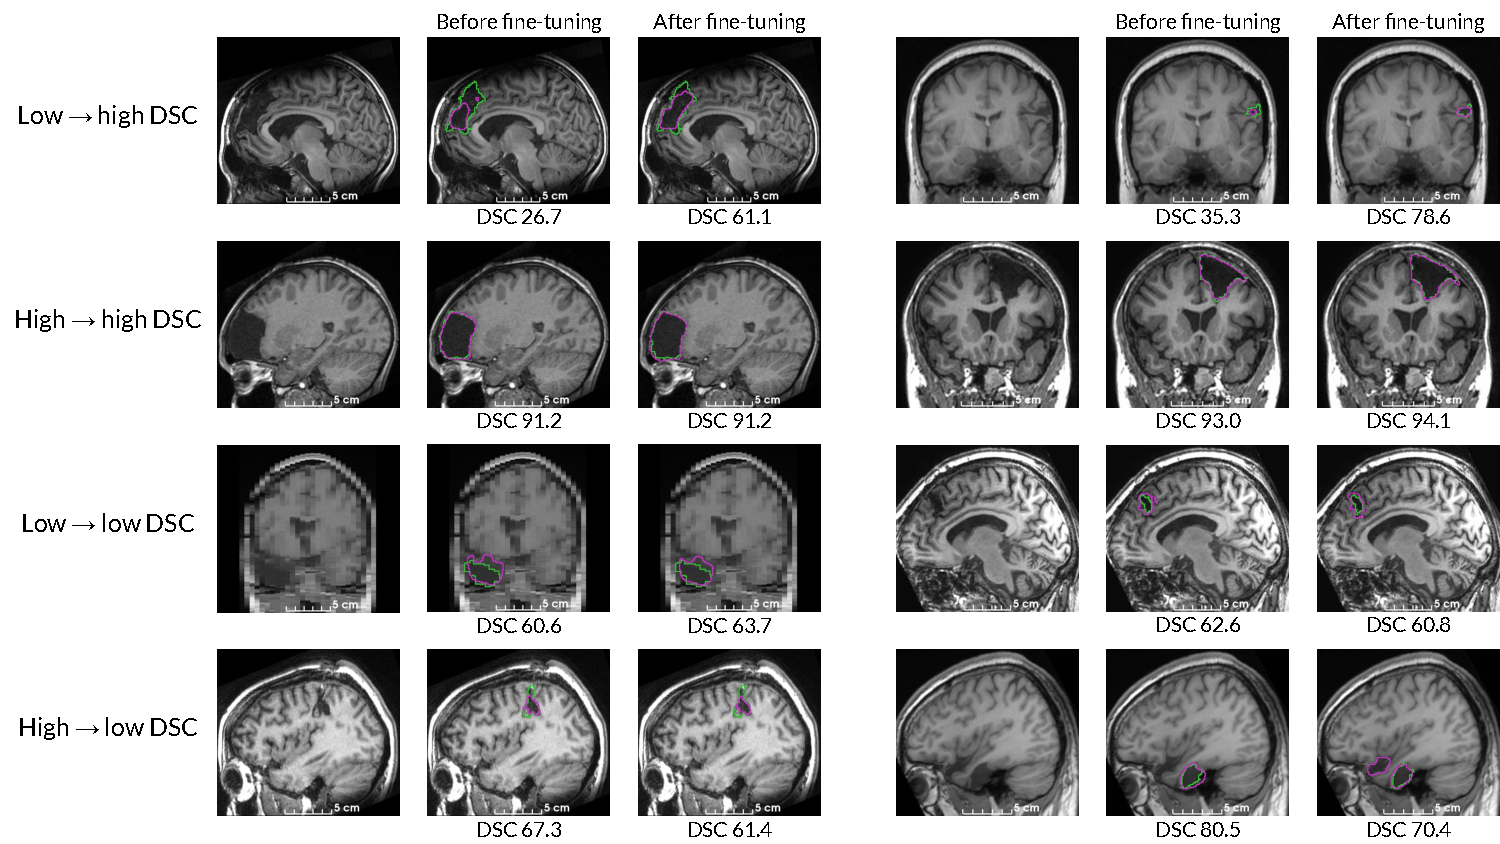
\includegraphics[width=\linewidth]{finetune}
  \caption{
      Qualitative evaluation of fine-tuning for the \textit{Strasbourg} (left) and EPISURG (right) datasets.
      Rows correspond, from top to bottom, to cases for which the \ac{DSC}
      1) increased,
      2) remained high,
      3) remained low and
      4) decreased
      after fine-tuning the self-supervised model.
      Manual annotations (green) and model predictions (magenta) are overlaid.
  }
  \label{fig:finetuning_qual}
\end{figure}

% \subsubsection{Semi-supervised learning: leveraging real unlabeled resections}
\label{sec:results_semi}

\newcommand{\pseudo}{\st{pseudo}}

In this experiment, we assessed the ability of semi-supervised learning to improve the performance of our baseline model.
We first computed the uncertainty $u(f_{\alpha\beta}, \X\post, n\st{unc})$ for $D\unl$ (\cref{sec:leveraging_semi}), all unlabeled images in EPISURG, using the baseline model and the preprocessing and augmentation transforms (\cref{sec:preprocessing_augmentation}).
We generated pseudolabels and estimated uncertainty from $n\st{unc} = 50$ Monte Carlo \ac{TTA} iterations (\cref{sec:leveraging_semi}).
To obtain the final dataset $D\pseudo = \{ (\X_{\text{postop}_i}, \wt{\Y}_{\text{cavity}_i}) \}_{i = 1}^{n\pseudo}$, we selected pseudolabels with $u(\X_{\text{postop}_i}, \cdot) < t\st{unc} = 0.2$, resulting in $n\pseudo = 256$.

We used $D\st{pre,train}$ (\cref{sec:self}) in addition to $D\pseudo$ to train a new model $\fp{sim,semi}(\cdot)$, using the same hyperparameters as in the self-supervised setting (\cref{sec:self}).
To ensure that all batches contain real resections, we use $b - b\pseudo$ images from $D\st{pre,train}$ and $b\pseudo$ images from $D\pseudo$ to compose each mini-batch of size $b$.
We chose $b\pseudo = 2$ for our experiments, i.e., 20\% of the images in each mini-batch contain real \acp{rc}.

Semi-supervised learning improved the performance of the baseline model from 80.5 (18.7) to 81.5 (17.8) ($p = 0.474$).


\begin{figure}
  \centering

  \begin{subfigure}{0.18\linewidth}
    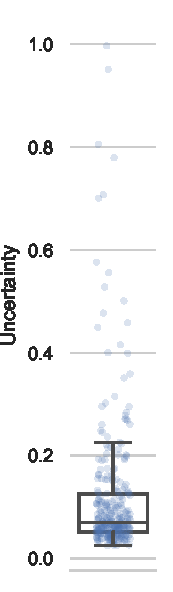
\includegraphics[width=\linewidth]{qcd}
    \caption{\label{fig:all_uncertainties}}
  \end{subfigure}
  \begin{subfigure}{0.194\linewidth}
    \begin{tabular}{c}
      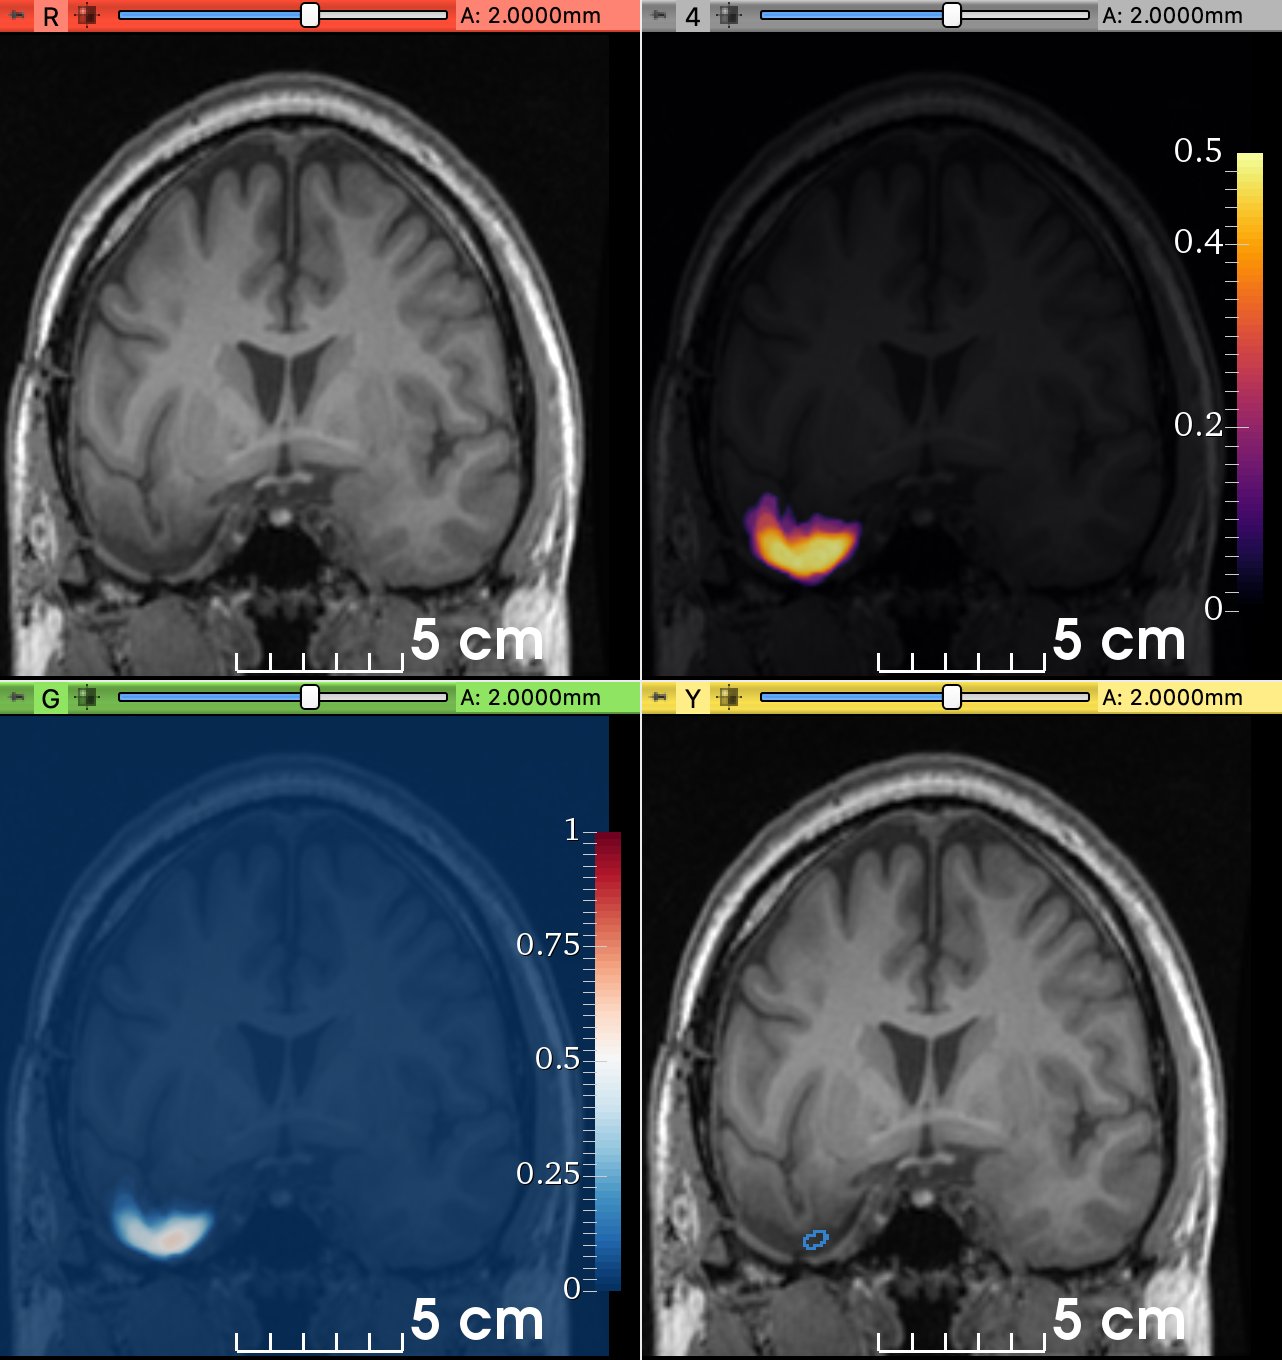
\includegraphics[trim=0 680 642 32, clip, width=\linewidth]{0796_uncertainty} \\
      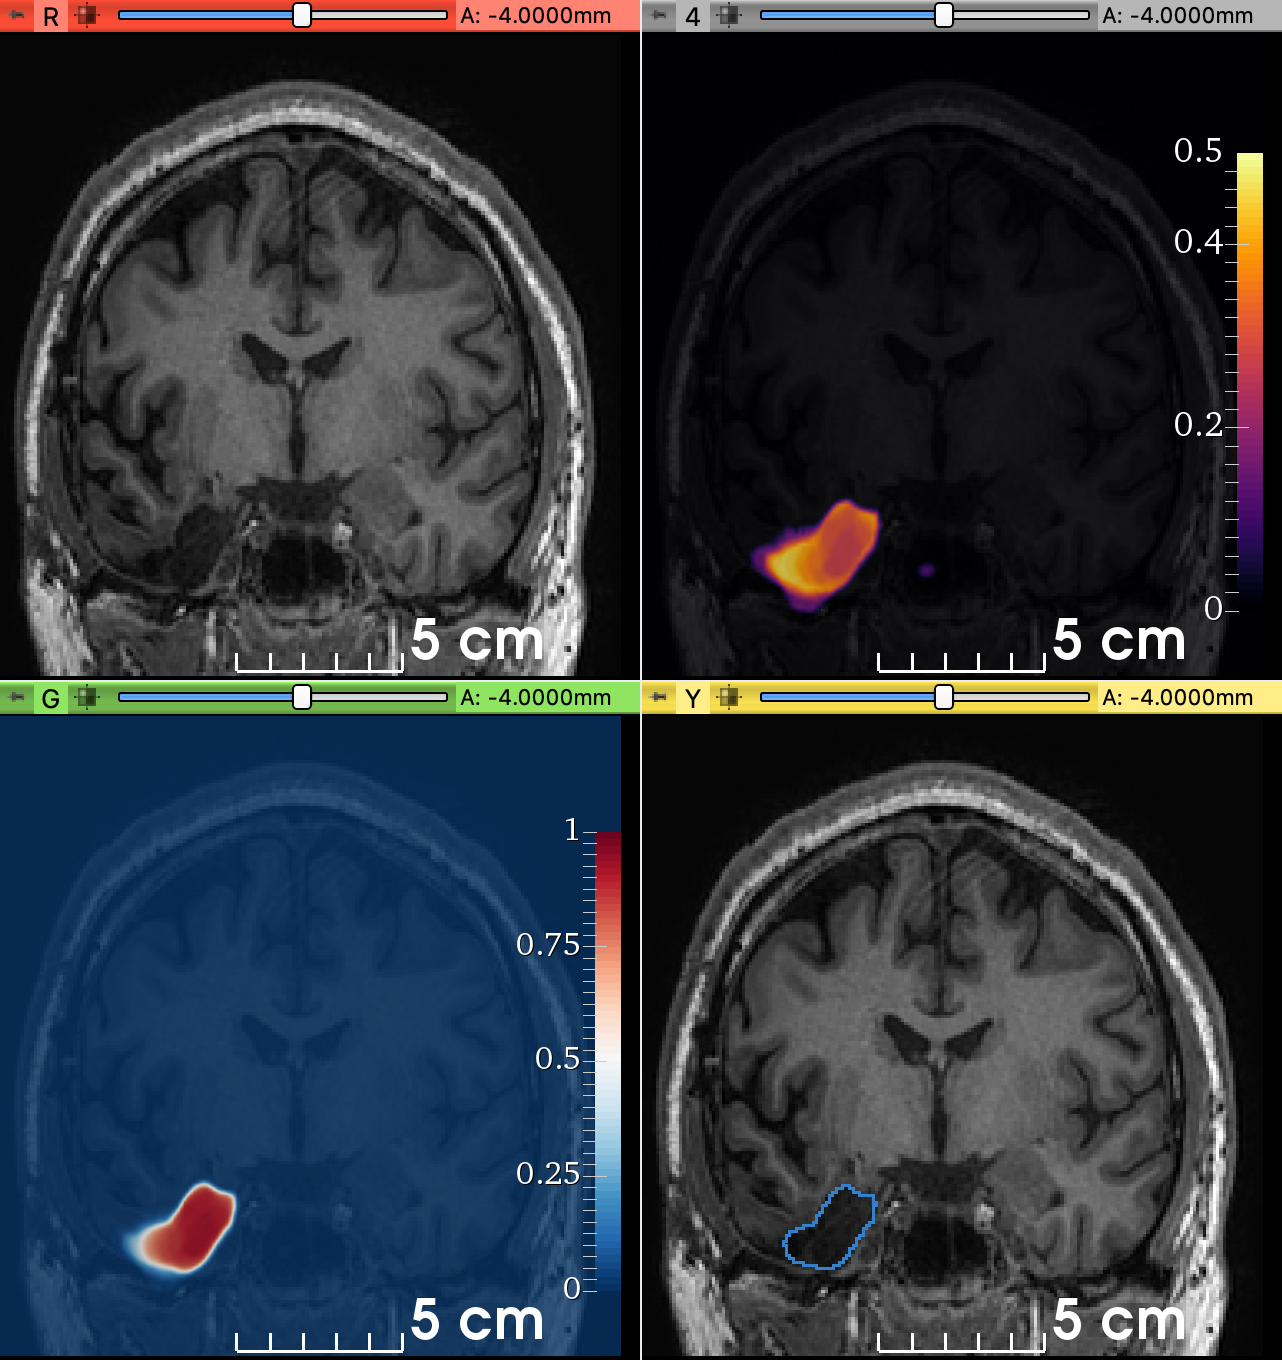
\includegraphics[trim=0 680 642 32, clip, width=\linewidth]{0914_uncertainty} \\
      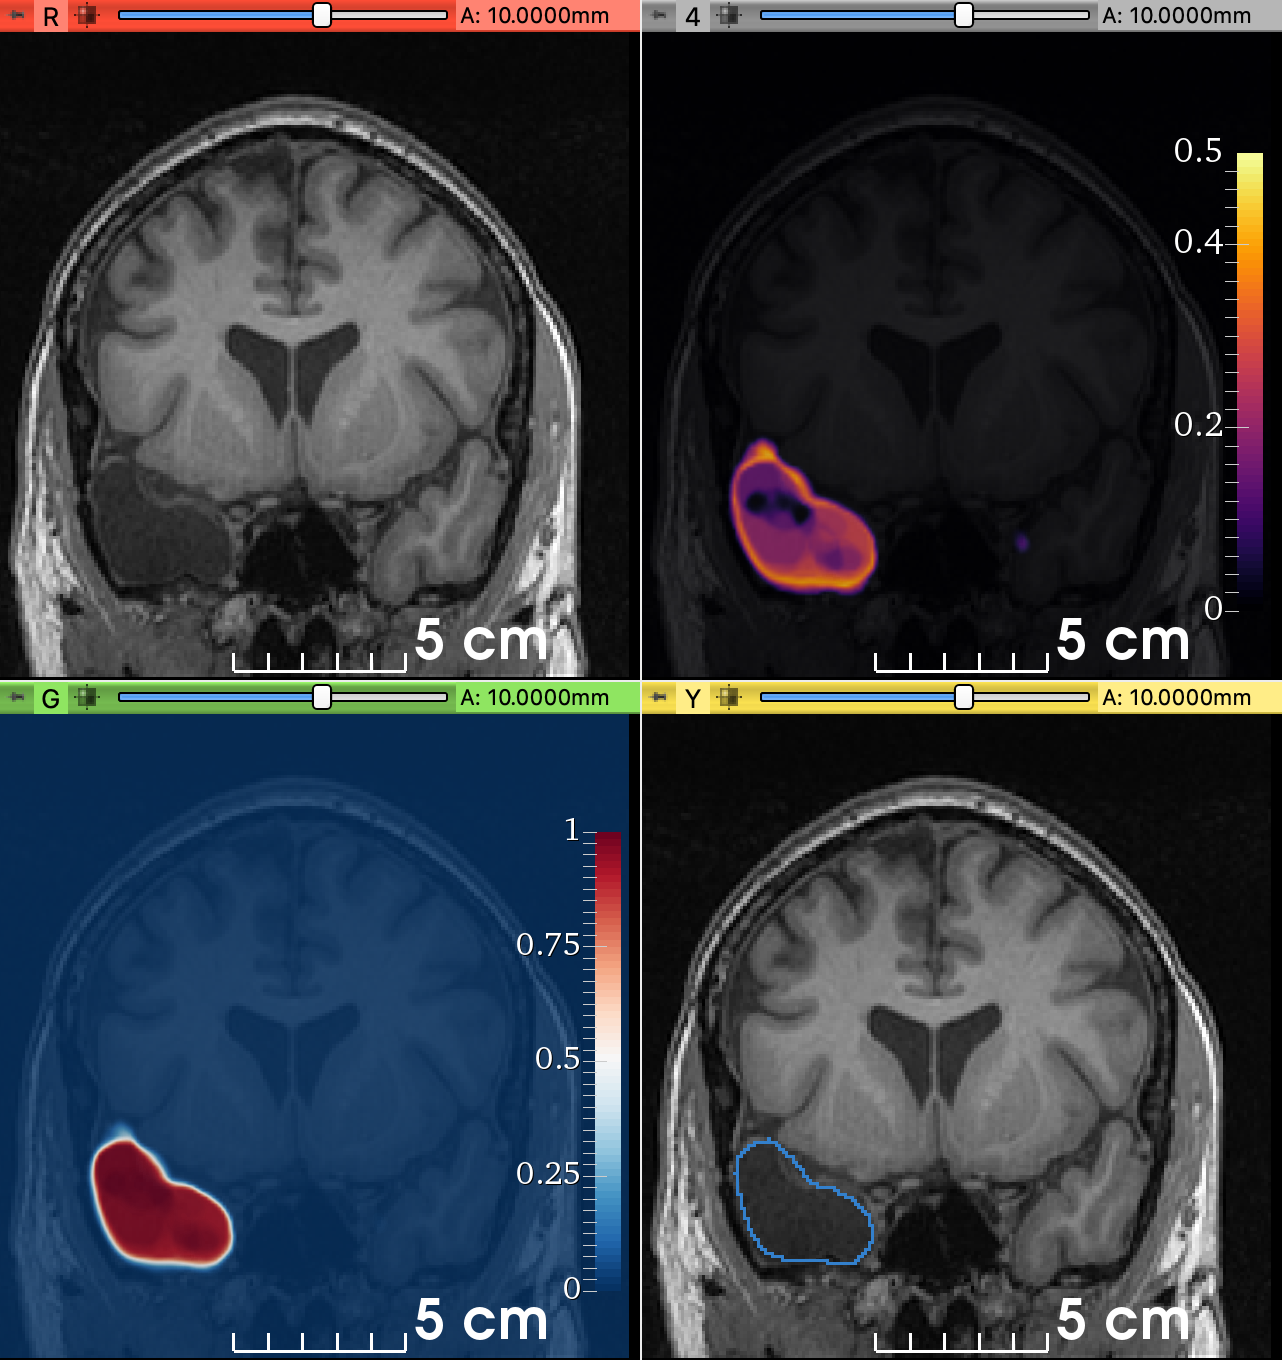
\includegraphics[trim=0 680 642 32, clip, width=\linewidth]{0499_uncertainty} \\
    \end{tabular}
    \caption{\label{fig:uncertainty_mri}}
  \end{subfigure}
  \begin{subfigure}{0.194\linewidth}
    \begin{tabular}{c}
      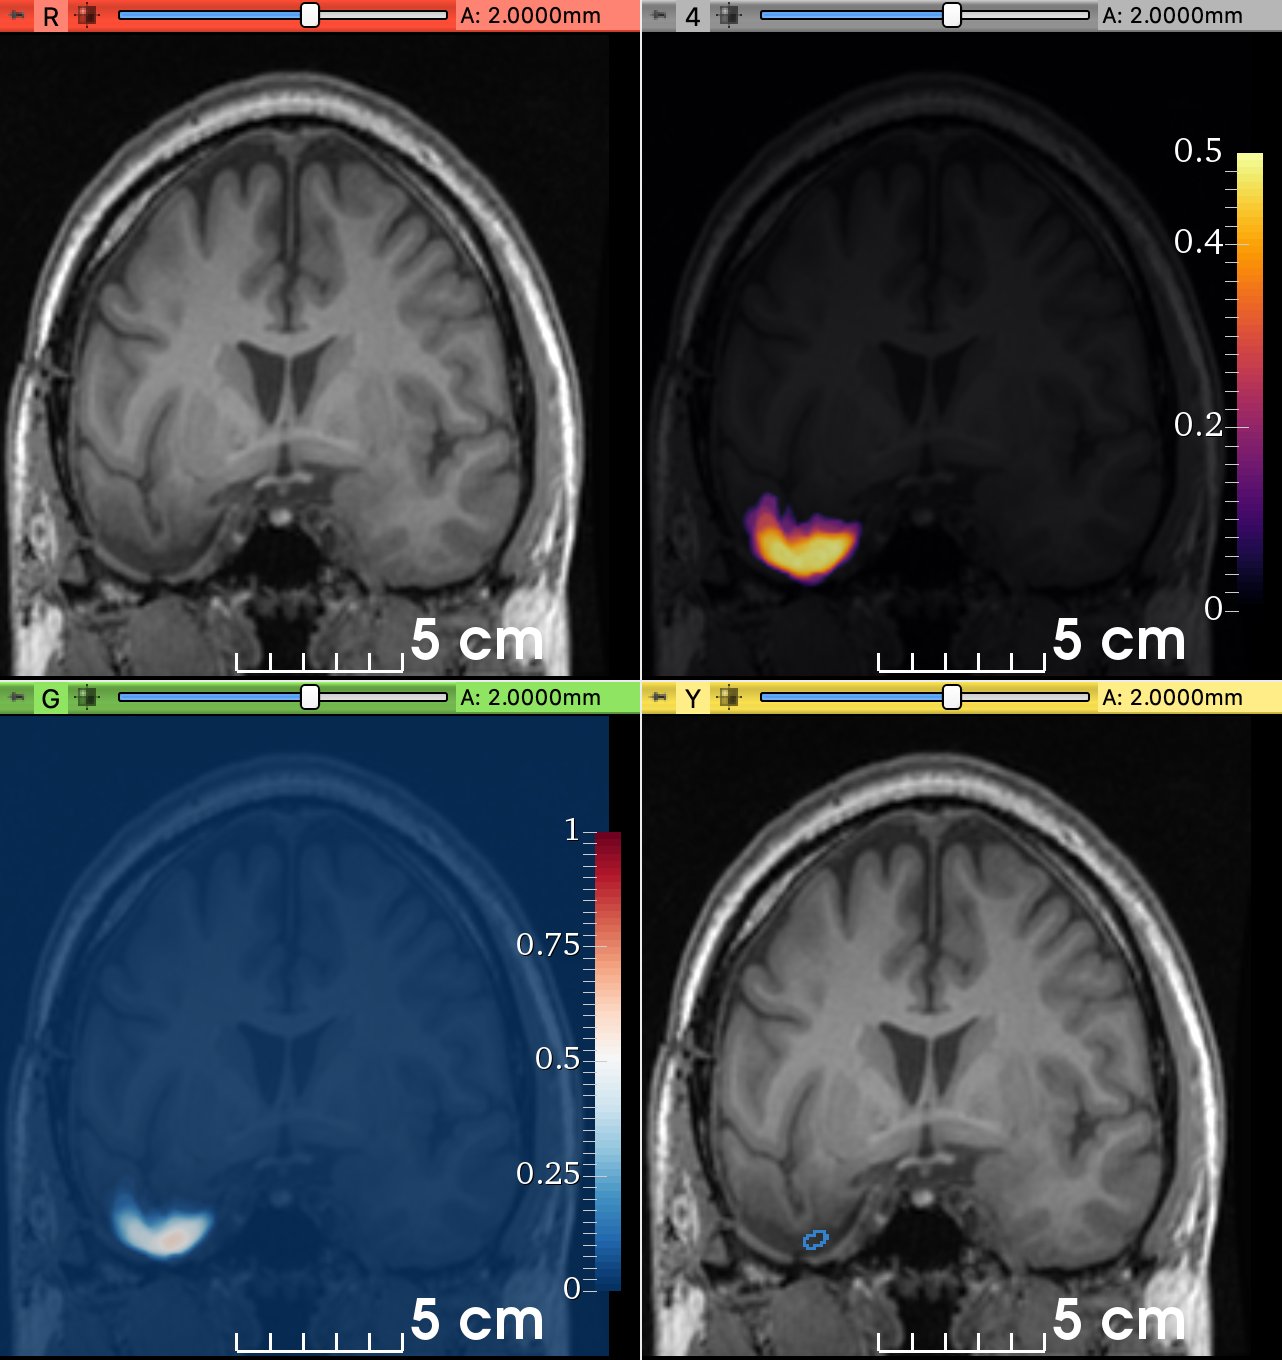
\includegraphics[trim=642 680 0 32, clip, width=\linewidth]{0796_uncertainty} \\
      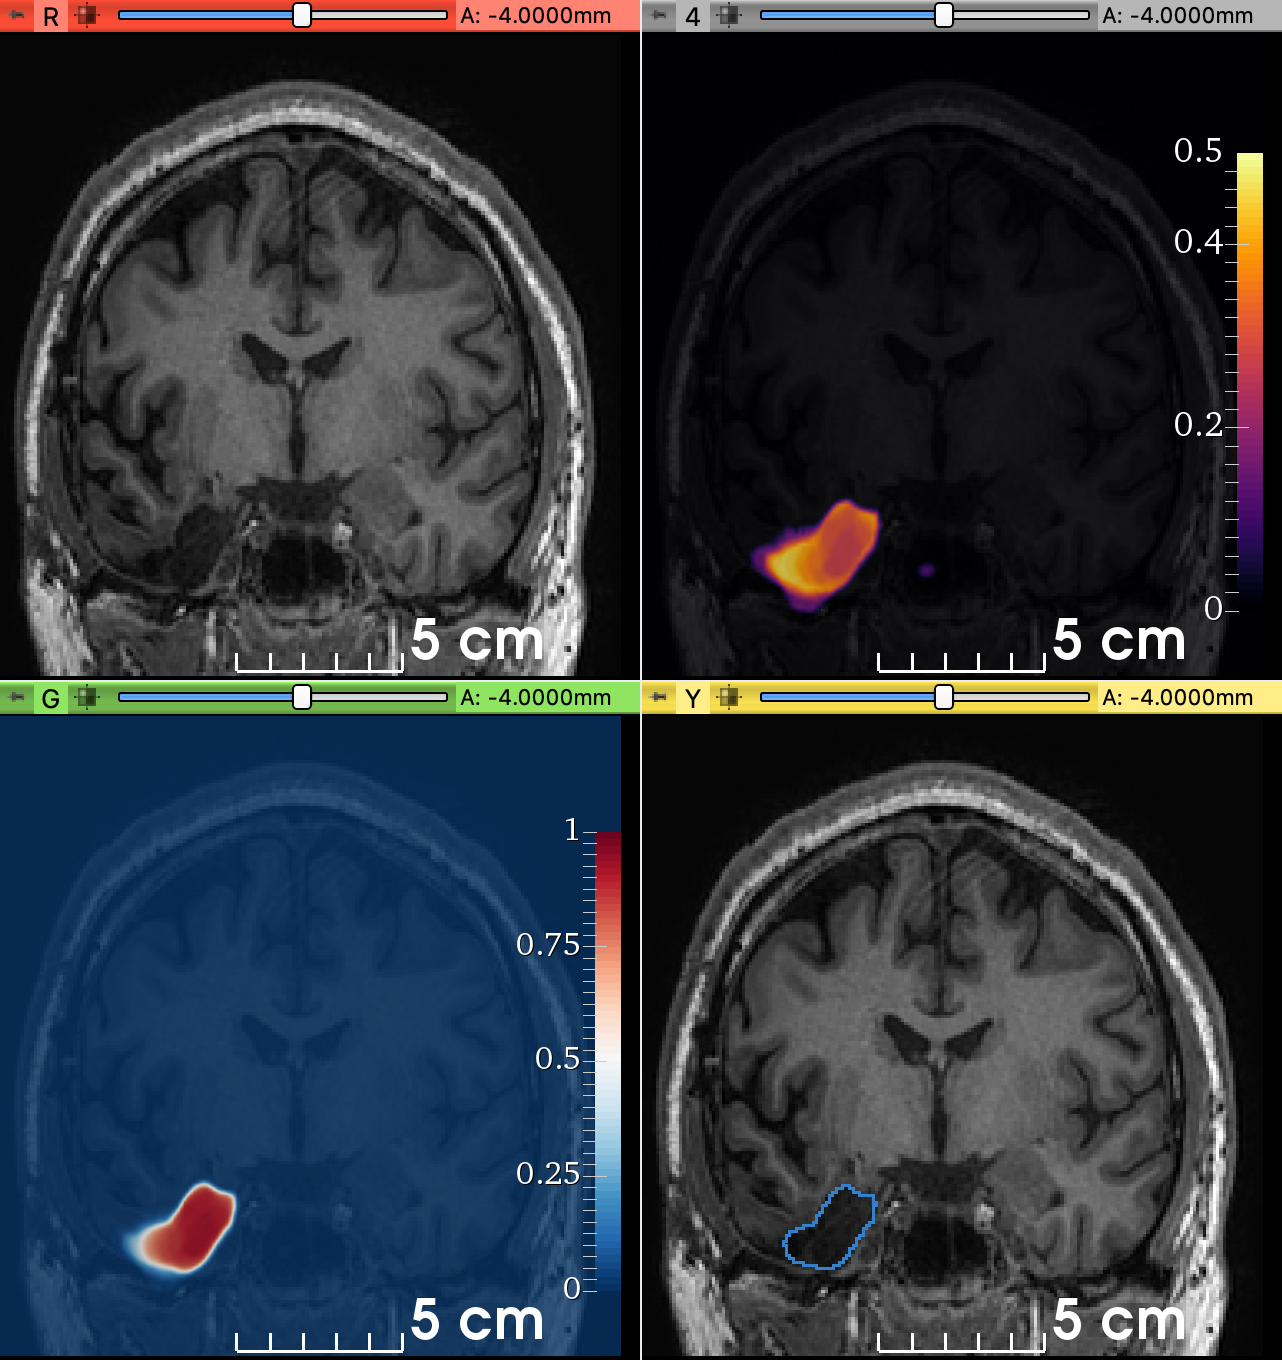
\includegraphics[trim=642 680 0 32, clip, width=\linewidth]{0914_uncertainty} \\
      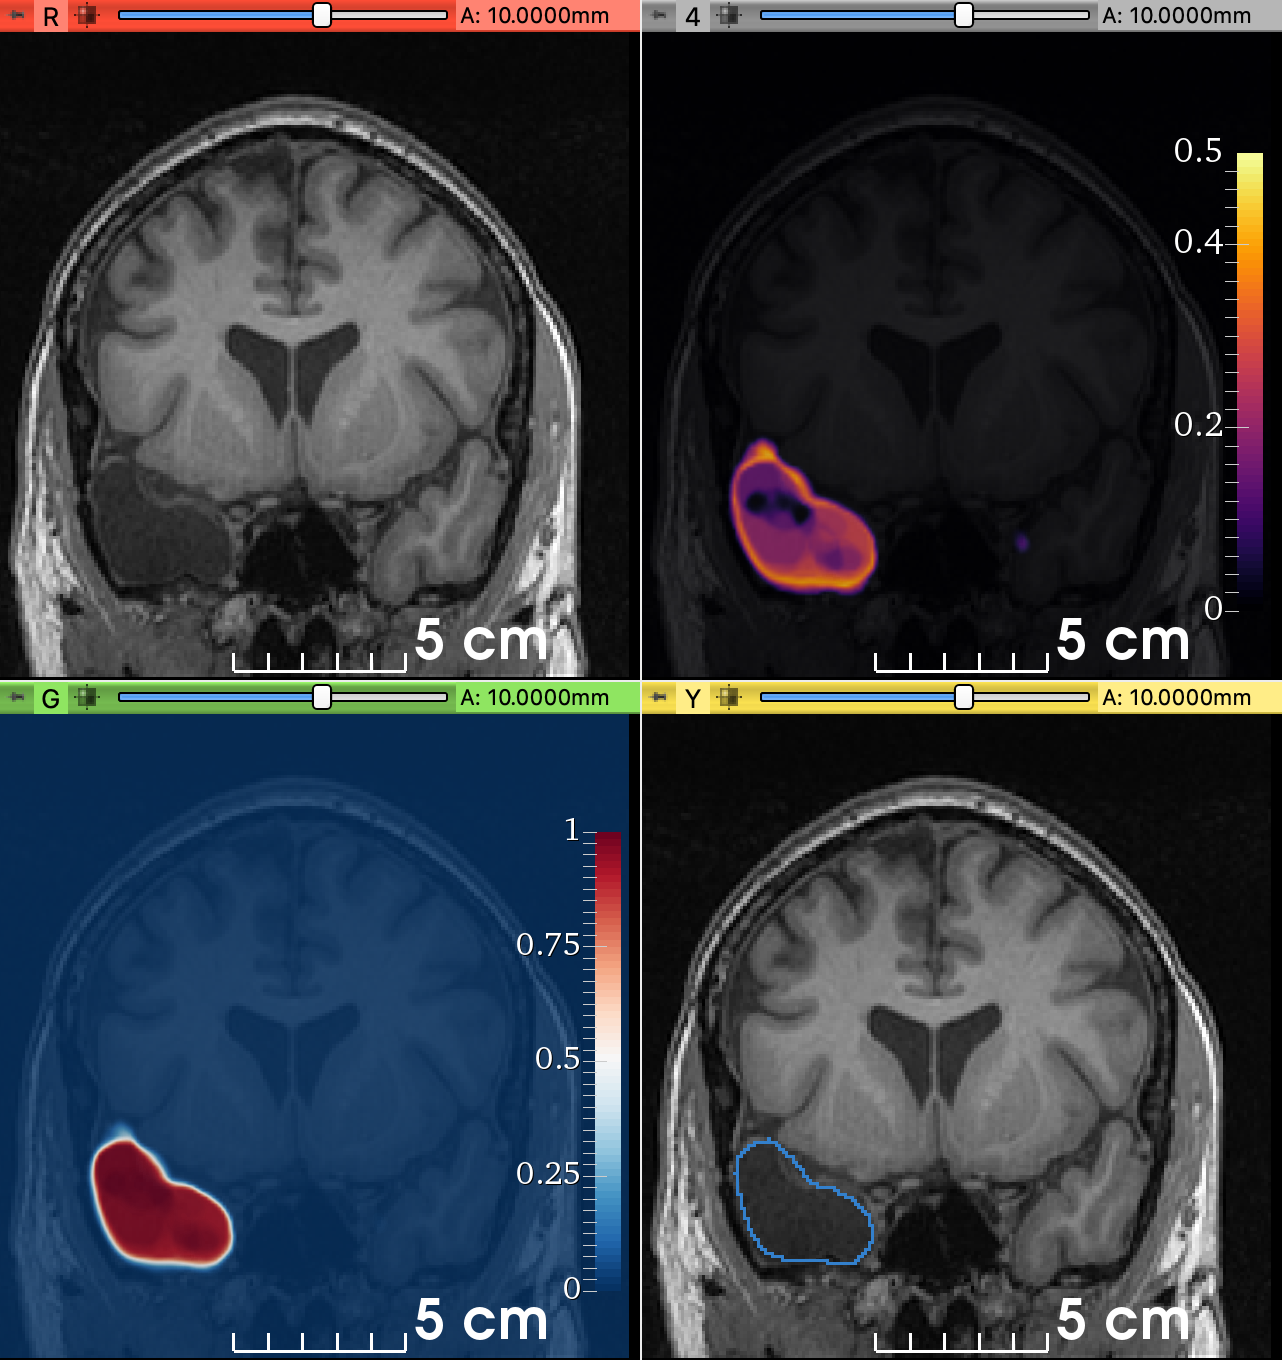
\includegraphics[trim=642 680 0 32, clip, width=\linewidth]{0499_uncertainty} \\
    \end{tabular}
    \caption{\label{fig:uncertainty_std}}
  \end{subfigure}
  \begin{subfigure}{0.194\linewidth}
    \begin{tabular}{c}
      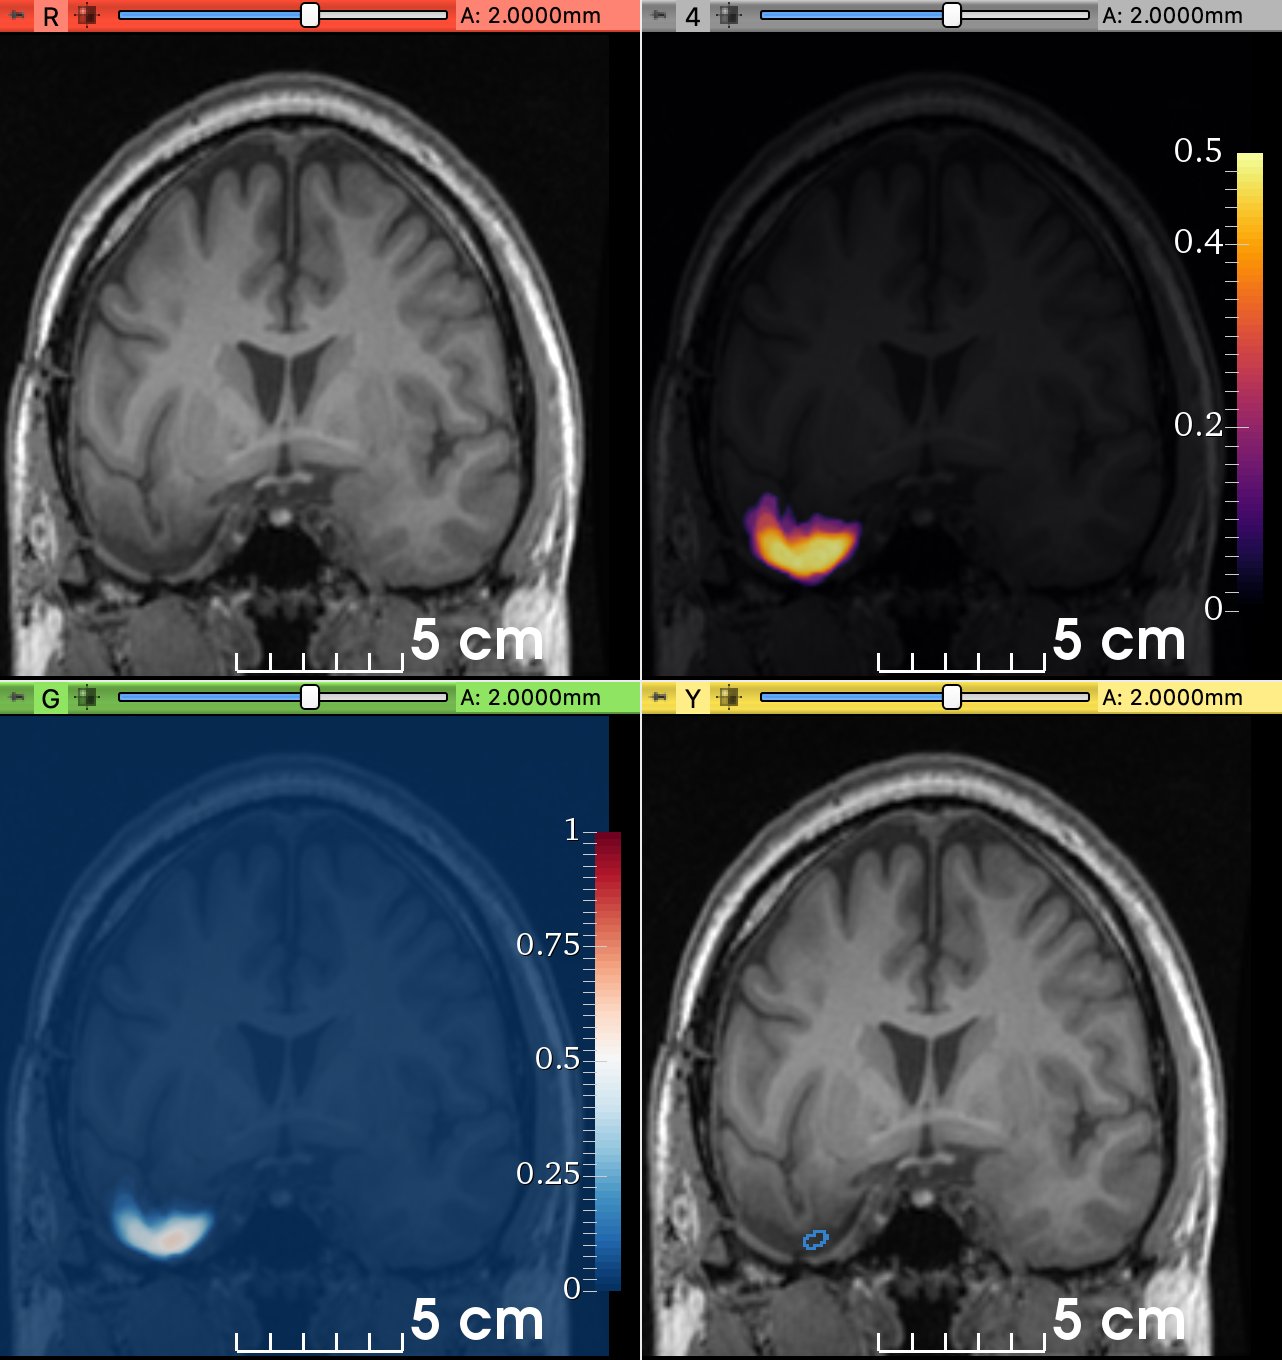
\includegraphics[trim=0 0 642 714, clip, width=\linewidth]{0796_uncertainty} \\
      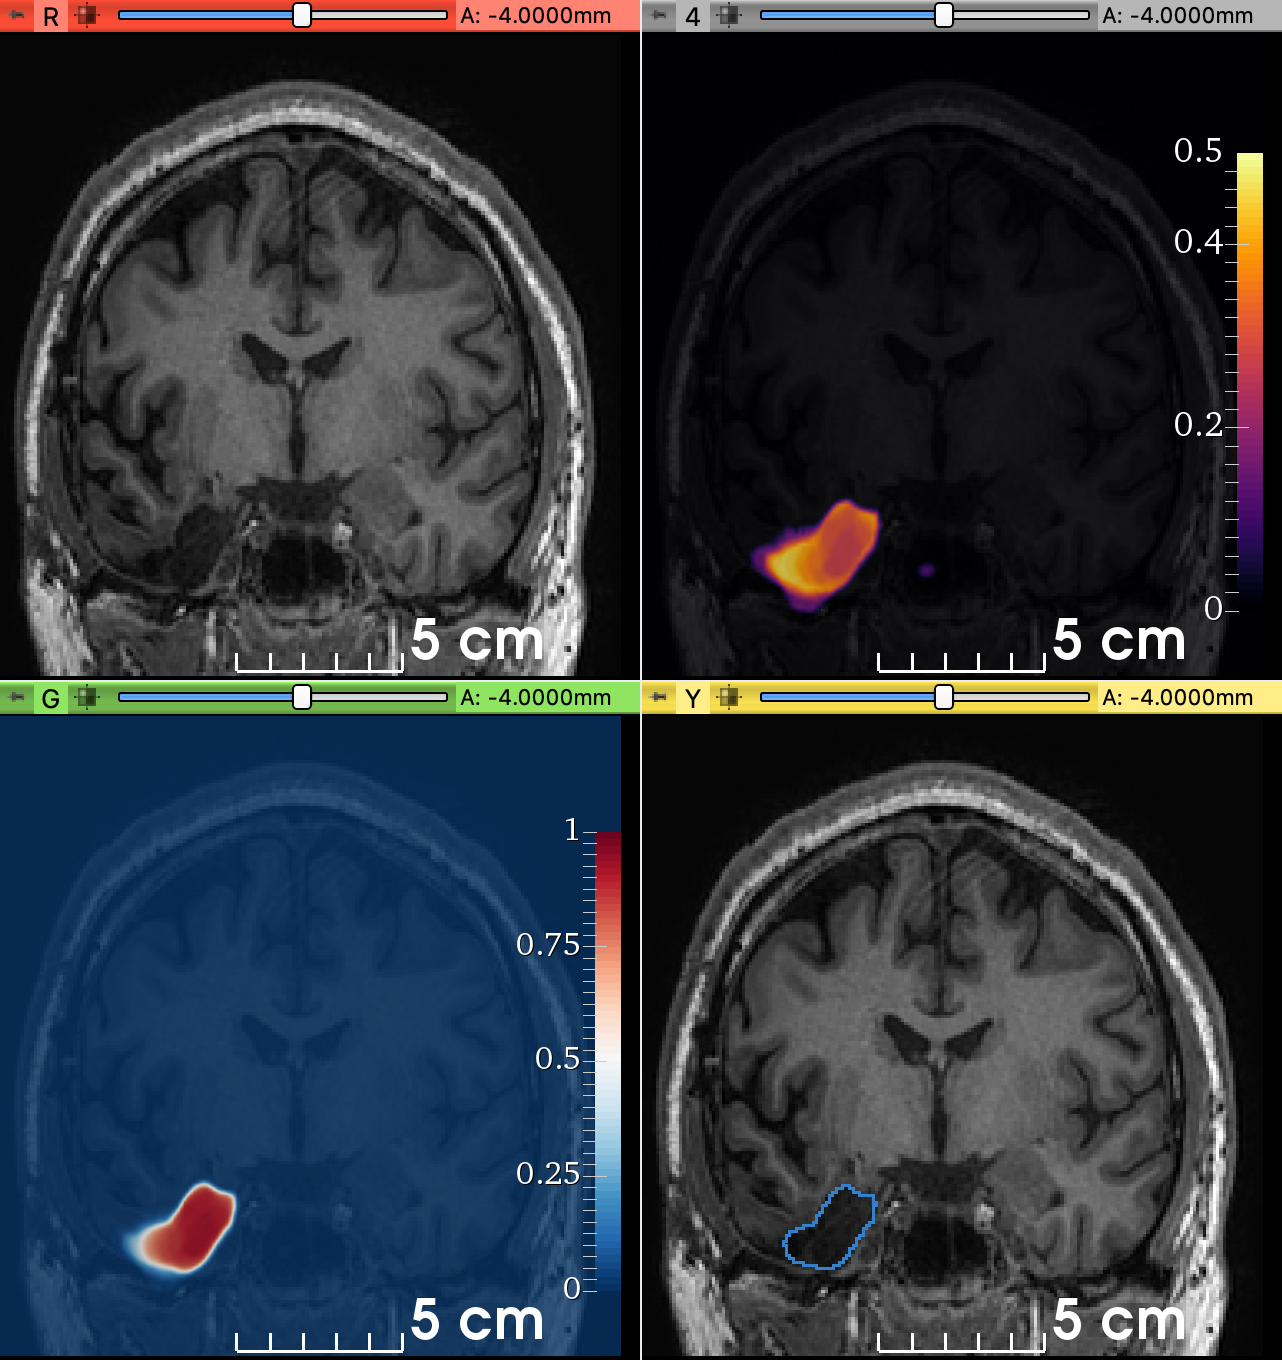
\includegraphics[trim=0 0 642 714, clip, width=\linewidth]{0914_uncertainty} \\
      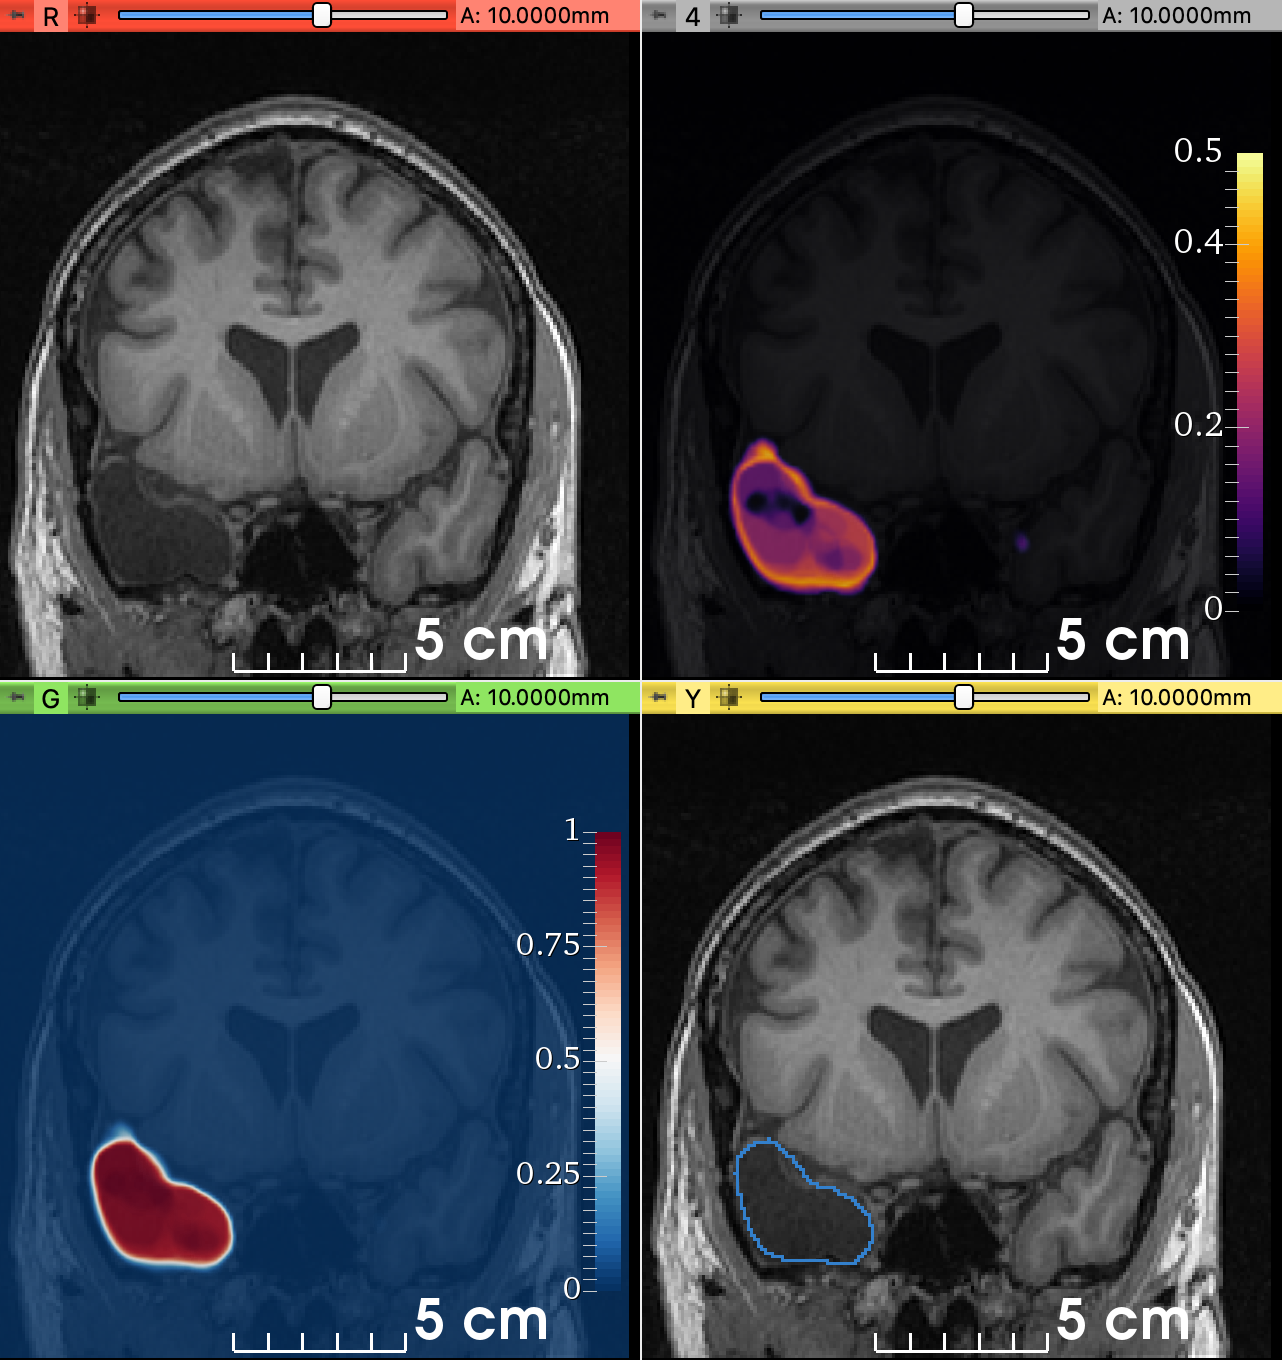
\includegraphics[trim=0 0 642 714, clip, width=\linewidth]{0499_uncertainty} \\
    \end{tabular}
    \caption{\label{fig:uncertainty_mean}}
  \end{subfigure}
  \begin{subfigure}{0.194\linewidth}
    \begin{tabular}{c}
      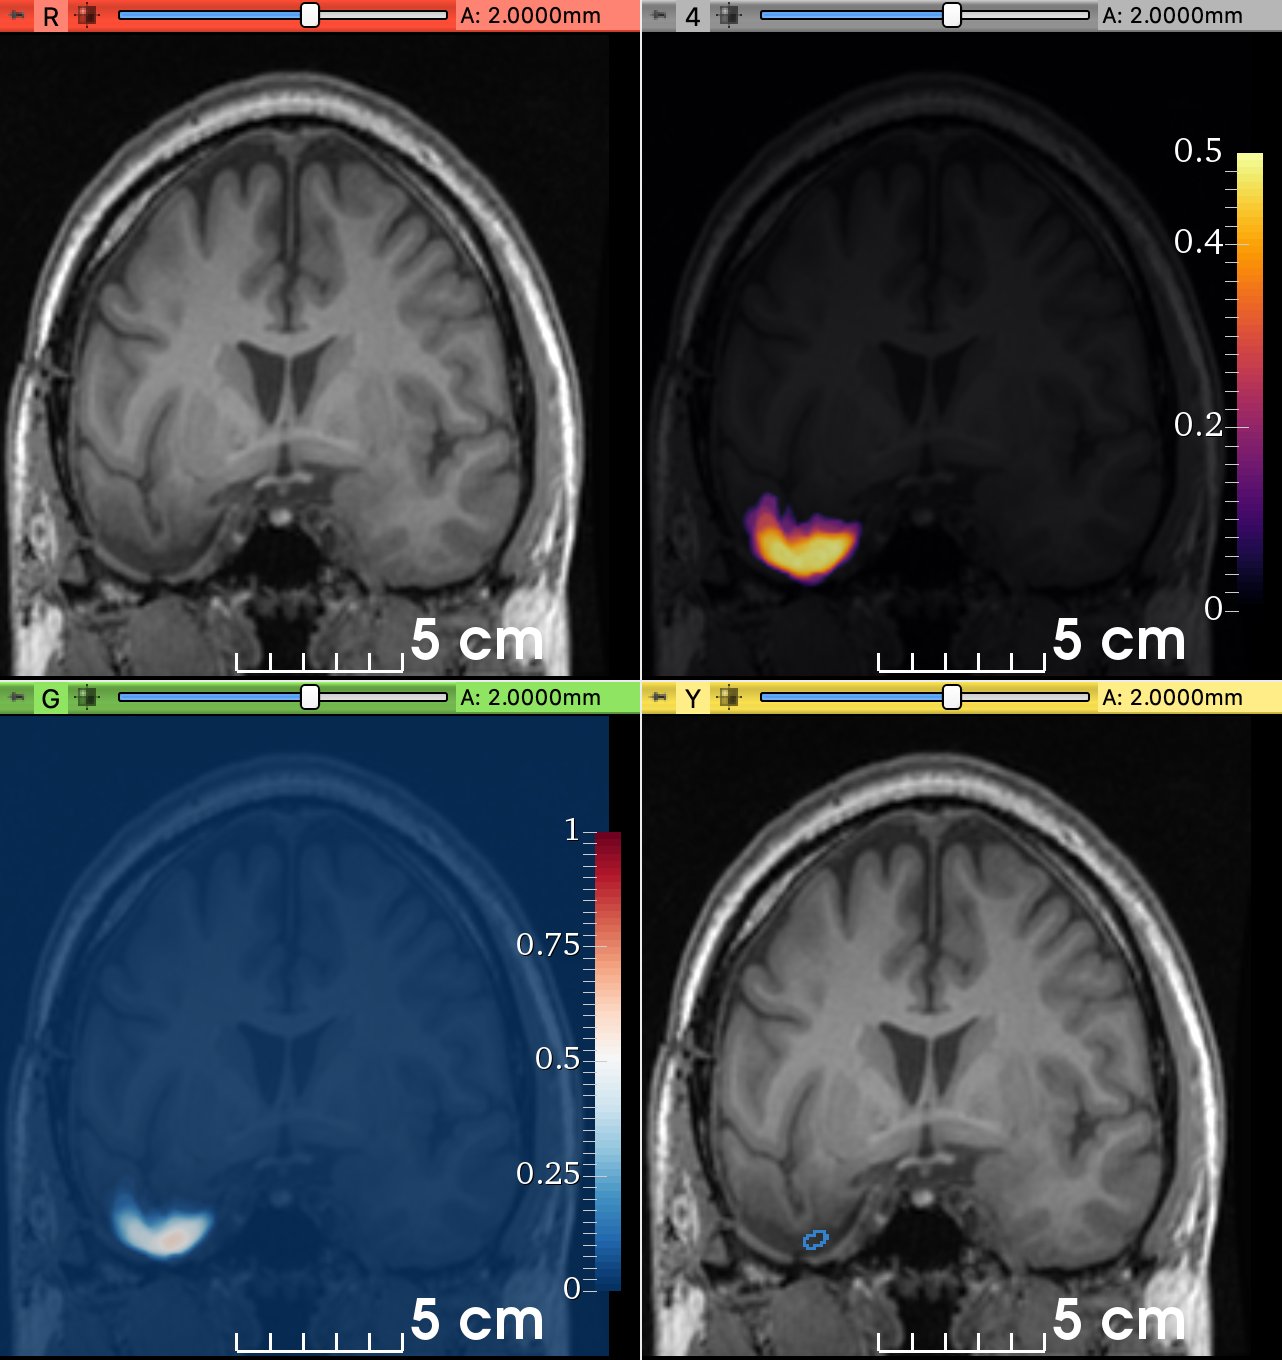
\includegraphics[trim=642 0 0 714, clip, width=\linewidth]{0796_uncertainty} \\
      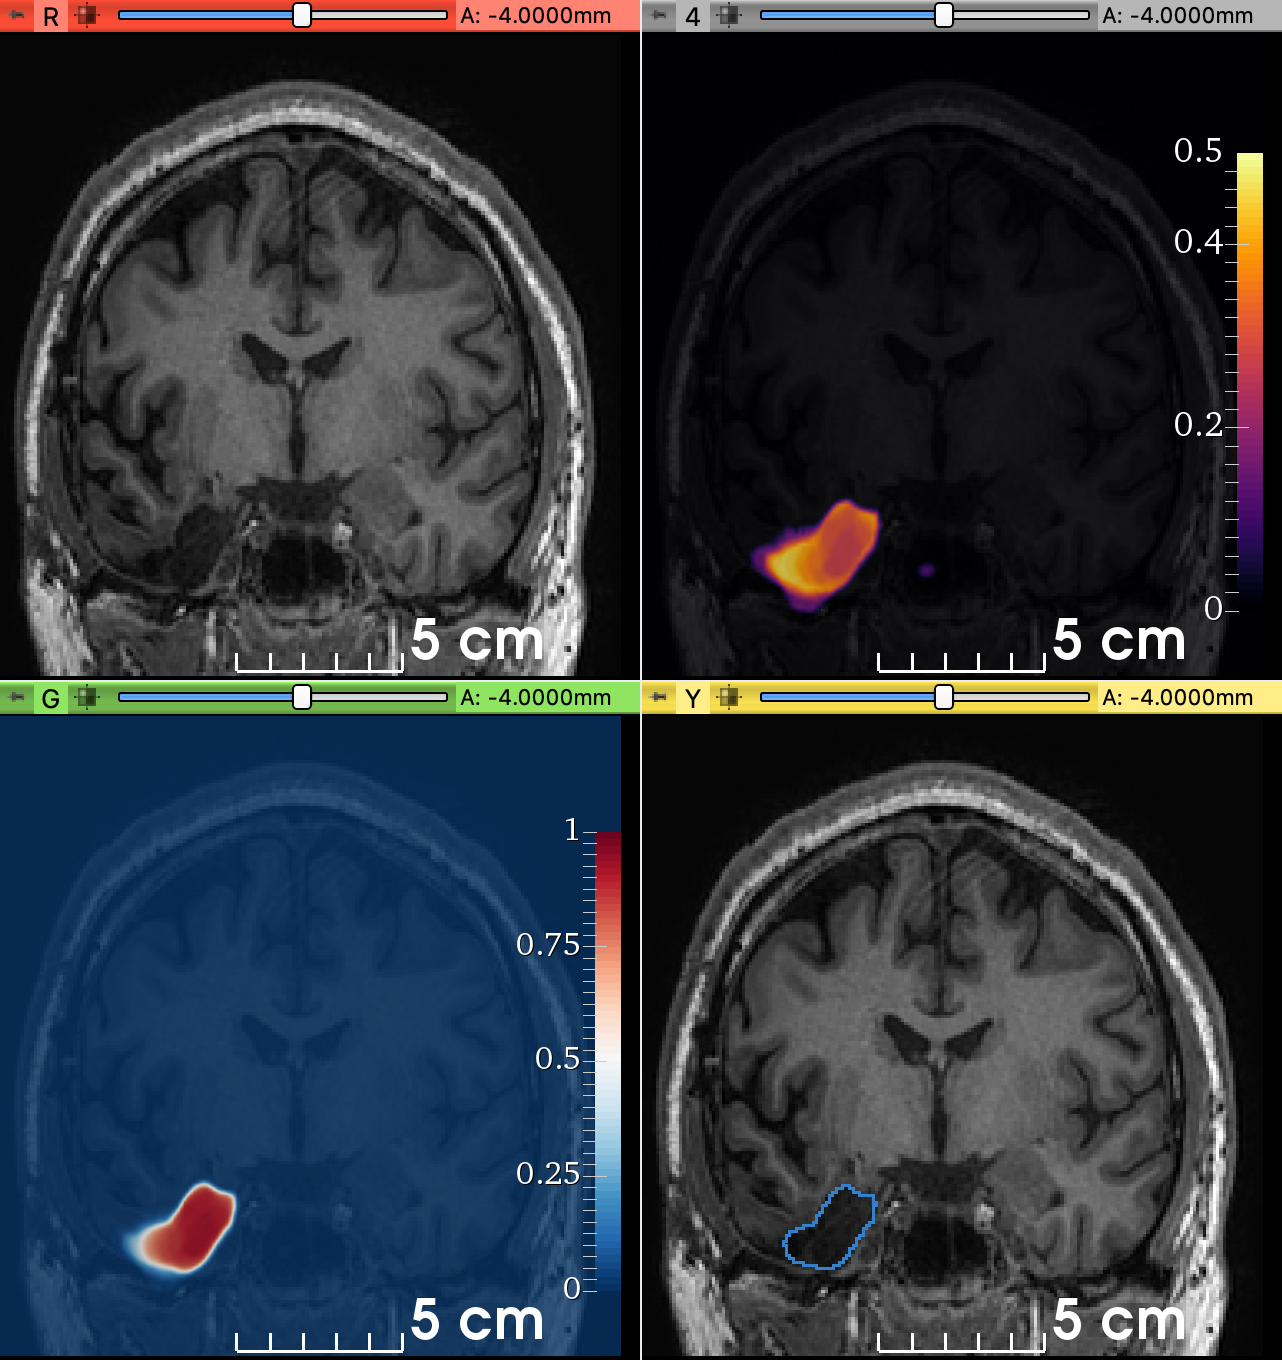
\includegraphics[trim=642 0 0 714, clip, width=\linewidth]{0914_uncertainty} \\
      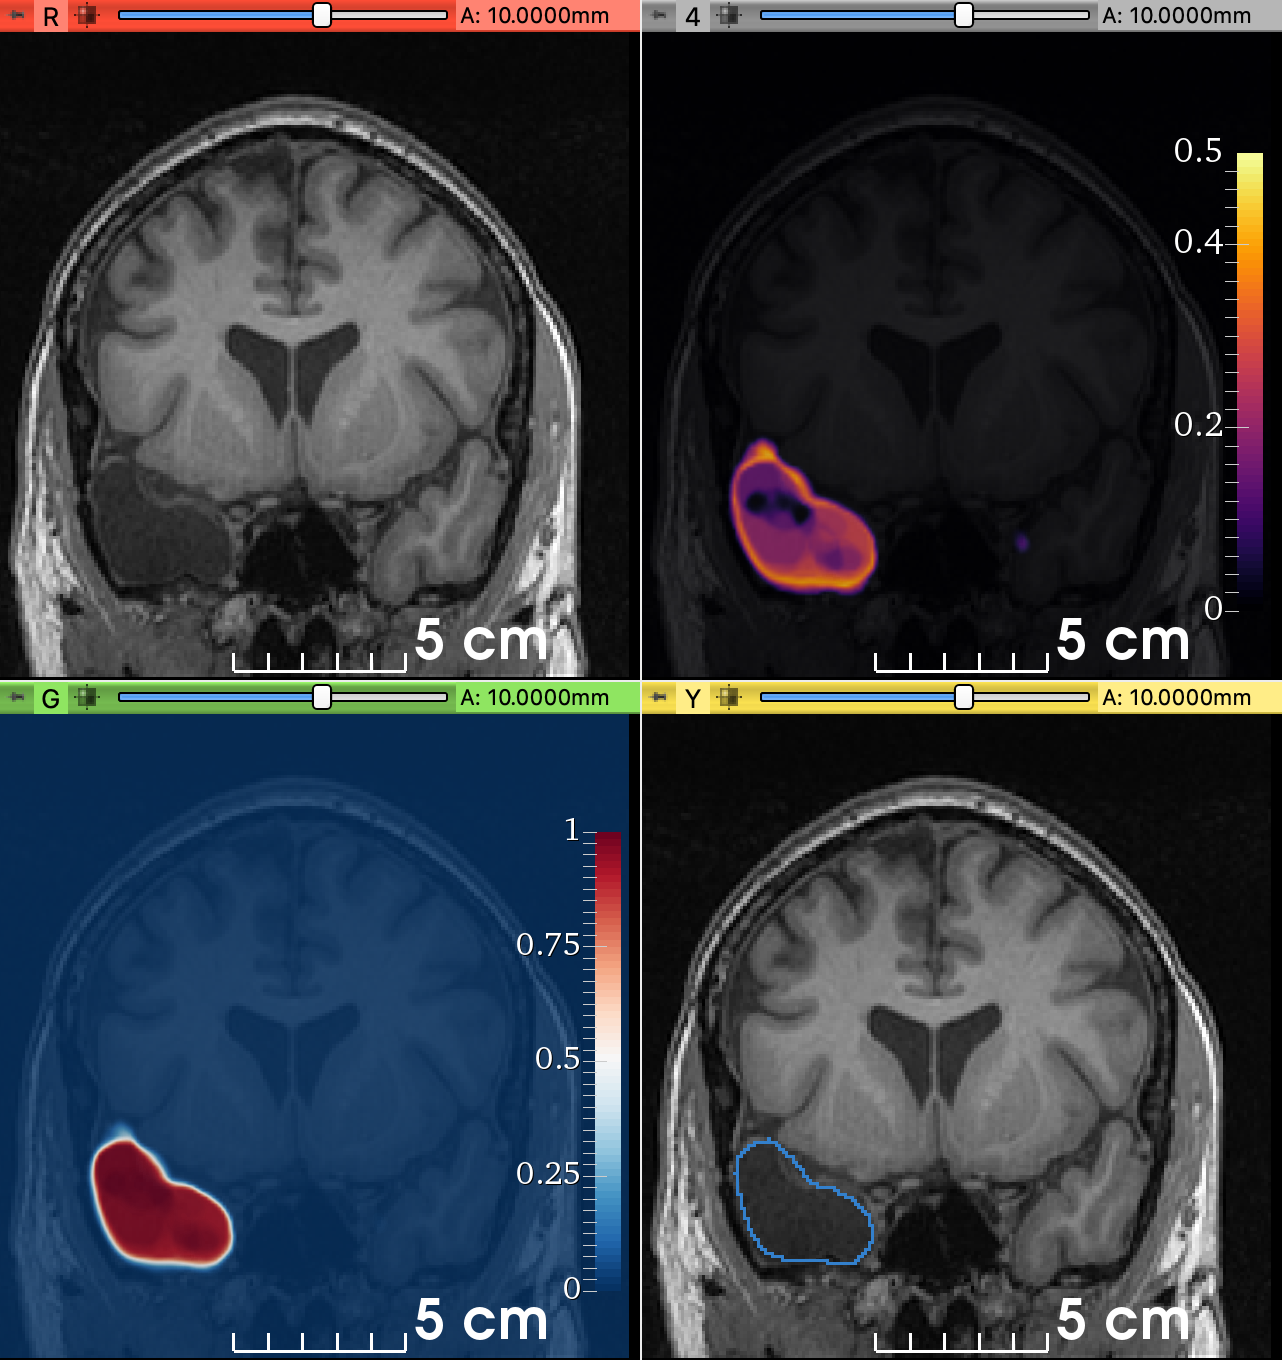
\includegraphics[trim=642 0 0 714, clip, width=\linewidth]{0499_uncertainty} \\
    \end{tabular}
    \caption{\label{fig:uncertainty_pseudo}}
  \end{subfigure}

  \caption[Generating reliable pseudolabels for semi-supervised learning]{
    Generating reliable pseudolabels for semi-supervised learning.
    Image-level uncertainty for the 297 unlabeled postoperative images in EPISURG (\subref{fig:all_uncertainties}).
    Unlabeled postoperative \ac{T1w} \ac{MRI} (\subref{fig:uncertainty_mri}).
    Voxel-wise uncertainty (\subref{fig:uncertainty_std}) estimated as the standard deviation of the probabilities across all Monte Carlo iterations.
    The mean prediction (\subref{fig:uncertainty_mean}) is thresholded at 0.5 to generate the pseudolabel (\subref{fig:uncertainty_pseudo}).
    Image-level uncertainties for the three cases are 0.805 (top), 0.195 (middle) and 0.025 (bottom).
  }
  \label{fig:uncertainties}
\end{figure}

% \subsubsection{Qualitative evaluation on brain tumor resection dataset}

We used the \ac{BITE} dataset \cite{mercier_online_2012} to evaluate the ability of our self-supervised model to segment \acp{RC} on images from a different institution, modality and pathology than the datasets used for quantitative evaluation.
For postprocessing, all but the largest binary connected component were removed.
The model successfully segmented the \ac{RC} on 11/13 images, even though some contained challenging features (\cref{fig:bite}).

\newcommand{\qualit}[1]{\includegraphics[width=0.14\linewidth]{bite/cropped/#1}}
\newcommand{\qualitfig}[1]{
  \centering
  \qualit{#1_sag}%
  \enskip
  \qualit{#1_seg_sag}%
  \quad
  \qualit{#1_cor}%
  \enskip
  \qualit{#1_seg_cor}%
  \quad
  \qualit{#1_axi}%
  \enskip
  \qualit{#1_seg_axi}
}

% https://tex.stackexchange.com/a/381477/216202
\begin{figure}
  \centering
  \begin{subfigure}{\textwidth}
    \qualitfig{2_low_contrast}
    \caption{Image with low contrast between the cavity and the brain \label{fig:bite_low_contrast}}
  \end{subfigure}
  \vskip\baselineskip
  \begin{subfigure}{\textwidth}
    \qualitfig{4_air}
    \caption{Image with air and CSF within the cavity \label{fig:bite_air}}
  \end{subfigure}
  \vskip\baselineskip
  \begin{subfigure}{\textwidth}
    \qualitfig{5_aniso}
    \caption{Image with a highly anisotropic voxel spacing \label{fig:bite_aniso}}
  \end{subfigure}
  \vskip\baselineskip
  \begin{subfigure}{\textwidth}
    \qualitfig{12_motion}
    \caption{Image with \ac{MRI} motion artifacts and adjacent edema \label{fig:bite_motion}}
  \end{subfigure}
  \caption{
    Qualitative evaluation of the self-supervised model on a dataset of postoperative brain tumor \ac{T1wCE} \ac{MRI}.
    The model is robust to multiple challenging scenarios:
    low contrast between the cavity and the brain (\subref{fig:bite_low_contrast}),
    air and \ac{CSF} within the resection cavity (\subref{fig:bite_air}),
    highly anisotropic voxel spacing (\subref{fig:bite_aniso}),
    motion artifacts and edema (\subref{fig:bite_motion}),
    and a different modality than used for training (all).
    Note that these images are from a different institution, modality and pathology than the datasets used for quantitative evaluation.
    Manual annotations are not available.
  }
  \label{fig:bite}
\end{figure}




\subsubsection{Qualitative evaluation on intraoperative image}

We used our baseline model to segment the \ac{RC} on one intraoperative \ac{MRI} from our institution.
Despite the large domain shift between the training dataset and the intraoperative image, which includes a retracted skin flap and a missing bone flap, the model was able to correctly estimate the \ac{RC}, discarding similar regions filled with \ac{CSF} or air (\cref{fig:intra}).

\begin{figure}
  \centering
  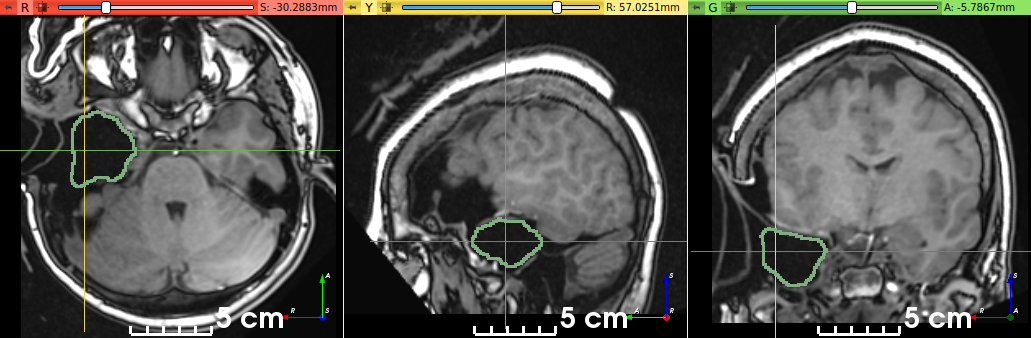
\includegraphics[trim=0 0 0 12, clip, width=\linewidth]{intra}
  \caption{
    Qualitative result on an intraoperative \ac{MRI}.
    The baseline model correctly discarded regions filled with air or \ac{CSF} outside of the \ac{RC}.
  }
  \label{fig:intra}
\end{figure}

